\subsection{World Driver}
To help us draw on the display, we made a class that, using the Nokia5110Driver, could render the entire game world from a char array. It was also used to draw the highscore- and intro screens. The class diagram for the World Driver can be seen on figure \ref{WorldDriverClassDiagram}.

\begin{figure}[H]
	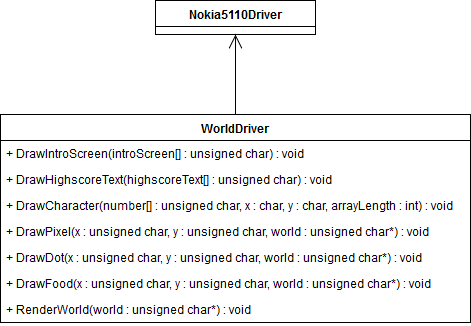
\includegraphics[width=8cm]{WorldDriverClassDiagram}
	\centering
	\caption{The class diagram for the WorldDriver.}
	\label{WorldDriverClassDiagram}
\end{figure}

The \textit{DrawIntroScreen, DrawHighscoreText}, and \textit{RenderWorld} methods all take an unsigned char array and sends it to the display for rendition.

The methods \textit{DrawDot}, \textit{DrawFood} and \textit{DrawPixel} does not send any data to the display themselves, but they populate the world array with 1's and 0's in the structure of the banks of the DDRAM (See section \ref{DisplaySection}). The dots, food and pixels are only rendered when the \textit{RenderWorld} method is called by the game loop.